%% VXR-Sandbox Applied Research Publication
%% Compile: pdflatex VXR_Sandbox_Paper.tex (×2)
\documentclass[conference]{IEEEtran}

\usepackage[T1]{fontenc}
\usepackage[utf8]{inputenc}
\usepackage{cite}
\usepackage{amsmath,amssymb,amsfonts}
\usepackage{graphicx}
\usepackage{textcomp}
\usepackage{xcolor}
\usepackage{booktabs}
\usepackage{multirow}
\usepackage{url}
\usepackage{balance}
\usepackage{microtype}
\usepackage{hyperref}

\hypersetup{
    colorlinks=true,
    linkcolor=blue!60!black,
    citecolor=blue!60!black,
    urlcolor=blue!70!black
}

\begin{document}

% --- Voxion Labs logo (broken-cube mark) ---
\begin{center}
    
\includegraphics[width=3cm]{Voxion_Labs_Logo.png}\\[0.4em]
    {\small\textit{Voxion Labs Applied Research Division}}
\end{center}

\title{VXR-Sandbox: Deterministic Linear Memory Isolation for Client-Side LLM Prompt Injection Defense}

\author{
\IEEEauthorblockN{Rudranarayan Jena}
\IEEEauthorblockA{\textit{Founder}\\
\textit{Voxion Labs}\\
Applied Research --- VXR-Sandbox\\
Email: research@voxionlabs.io}
}

\maketitle

\begin{abstract}
Large language model (LLM) deployments increasingly accept untrusted natural-language input at the application boundary, exposing system prompts, tool routers, and safety policies to \emph{prompt injection} and \emph{jailbreak} attacks. Cloud-hosted pre-inference filters introduce latency, data residency risk, and an expanded trust perimeter. We present \textbf{VXR-Sandbox}, a browser-native reference architecture that executes heuristic prompt-injection detection inside a WebAssembly (Wasm) module backed by a modern C++ kernel. The design enforces a \emph{deterministic linear-memory contract}: the hot-path analyzer operates exclusively over \texttt{std::string\_view} slices and \texttt{constexpr} static pattern tables, avoiding dynamic heap growth and JavaScript garbage-collection interference. A zero-backend JavaScript bridge marshals UTF-8 across the Wasm boundary with explicit \texttt{\_free} discipline on input buffers only. Empirical telemetry over 10{,}000 synthetic injection attempts demonstrates median Wasm scan latencies on the order of tens of microseconds versus millisecond-scale remote Python API guards, while preserving offline operability after initial module fetch. VXR-Sandbox is released as applied research by Voxion Labs to study security--performance--accessibility trade-offs in client-side LLM hardening.
\end{abstract}

\begin{IEEEkeywords}
Prompt injection, jailbreak defense, WebAssembly, linear memory, zero-backend security, LLM safety, applied research
\end{IEEEkeywords}

\section{Introduction}
\label{sec:intro}

Enterprise and consumer LLM integrations routinely concatenate user-supplied text with privileged \emph{system prompts}, retrieval-augmented generation (RAG) context, and agent tool specifications. Adversaries embed override phrases---\emph{``ignore previous instructions''}, persona hijacks (\emph{``you are a DAN''}), or exfiltration requests---to subvert downstream model behavior~\cite{liu2024prompt,perez2022ignore}. Mitigations span model fine-tuning, constitutional classifiers, and external policy engines; however, many production stacks still rely on regex-heavy pre-filters or remote moderation APIs executed \emph{before} tokenization.

Three systemic frictions motivate client-side Wasm isolation:

\begin{enumerate}
    \item \textbf{Data residency}: Routing prompts to third-party APIs duplicates sensitive content across jurisdictional boundaries.
    \item \textbf{Tail latency}: WAN round-trips dominate P99 guard latency under load spikes.
    \item \textbf{Runtime nondeterminism}: JavaScript-only heuristics contend with V8 garbage-collection (GC) pauses, complicating real-time UX budgets in embedded chat widgets.
\end{enumerate}

\textbf{VXR-Sandbox} (Voxion eXperimental Research---Sandboxing) addresses these constraints through a \emph{zero-backend} pipeline: vanilla HTML/CSS/JavaScript UI, an Emscripten-compiled C++17 kernel (\texttt{analyze\_prompt}), and static deployment to GitHub Pages. This paper formalizes the threat model, describes the Wasm linear-memory architecture, and reports telemetry comparing local Wasm execution against representative remote Python API guards.

\section{Threat Model}
\label{sec:threat}

We consider an adversary $\mathrm{Adv}$ who supplies a bounded-length UTF-8 string $p \in \Sigma^\ast$ to a web-hosted chat surface. The defender runtime $\mathrm{Def}$ concatenates $p$ with a secret system prompt $s$ and optional tool schema $\tau$. $\mathrm{Adv}$'s objective is one of:

\begin{itemize}
    \item \textbf{Instruction override} ($\mathcal{O}$): induce $\mathrm{Def}$ to prioritize instructions embedded in $p$ over $s$.
    \item \textbf{Policy bypass} ($\mathcal{B}$): disable refusals, moderation, or rate limits.
    \item \textbf{Prompt exfiltration} ($\mathcal{E}$): recover $s$ or $\tau$ via model output.
    \item \textbf{Persona redefinition} ($\mathcal{P}$): force alternate role-play personas (e.g., ``Do Anything Now'' variants).
\end{itemize}

We assume $\mathrm{Adv}$ controls $p$ only (not Wasm bytecode, not browser DevTools in our honest-but-curious baseline). Supply-chain compromise of the Wasm artifact is out of scope but noted in Section~\ref{sec:conclusion}.

Detection is \emph{pre-inference}: a function $f_\theta(p) \rightarrow (\text{safe}, \ell, r)$ where $\ell \in [1,10]$ is threat level and $r$ a machine-readable reason code. False negatives arise from paraphrase and encoding attacks; false positives from benign educational text. VXR-Sandbox Phase~1 implements lexical heuristics $f_\theta$ as a static pattern library $\mathcal{P} = \{(k_i, w_i, \rho_i)\}$ with keyword $k_i$, weight $w_i$, and reason $\rho_i$.

\begin{table}[t]
\centering
\caption{Representative Jailbreak Heuristic Classes in VXR-Sandbox Phase~1}
\label{tab:patterns}
\begin{tabular}{@{}llc@{}}
\toprule
\textbf{Class} & \textbf{Example trigger} & \textbf{$w_i$} \\
\midrule
Instruction override & ``ignore previous instructions'' & 9 \\
System override & ``system override'' & 10 \\
Bypass language & ``bypass safety'' & 9 \\
Persona hijack & ``you are a / pretend you are'' & 5--6 \\
DAN variant & ``do anything now'' / word ``dan'' & 8--9 \\
Exfiltration & ``reveal system prompt'' & 9 \\
\bottomrule
\end{tabular}
\end{table}

\section{Related Work and Zero-Backend Positioning}
\label{sec:related}

Cloud moderation APIs (e.g., OpenAI Moderation~\cite{openai2024}) and hosted guardrails provide semantic classification at the cost of network dependency and prompt duplication. Browser extensions and enterprise proxies intercept traffic but rarely offer reproducible open kernels for academic audit. VXR-Sandbox occupies a distinct point in the design space: \emph{fully client-side}, \emph{open C++ source}, and \emph{statically deployable} without TLS-terminated ingress.

Compared to pure JavaScript regex guards, Wasm+C++ yields:
\begin{itemize}
    \item predictable instruction-level performance under V8 GC;
    \item compact binary artifacts cacheable via CDN Service Workers;
    \item a migration path toward fixed-arena ONNX inference without leaving the browser.
\end{itemize}

Compared to server-side Python stacks, zero-backend deployment eliminates cold-start variance of multi-tenant API pools and removes IAM/API-key onboarding for research demos---a deliberate accessibility choice for Voxion Labs field workshops.

\section{Wasm Linear Memory Architecture}
\label{sec:arch}

\subsection{Design Invariants}

The C++ kernel maintains four invariants during \texttt{analyze\_prompt}:

\begin{enumerate}
    \item[I1.] \textbf{No heap allocation in the hot loop} --- patterns are \texttt{constexpr HeuristicPattern kPatterns[]}.
    \item[I2.] \textbf{Non-owning views} --- input is scanned as \texttt{std::string\_view(prompt)} without copy.
    \item[I3.] \textbf{Static serialization buffer} --- JSON output is written to \texttt{g\_result\_buffer[512]} in \texttt{.bss}.
    \item[I4.] \textbf{Explicit JS/Wasm ownership} --- only the UTF-8 \emph{input} pointer allocated by \texttt{stringToNewUTF8} is \texttt{\_free}'d from JavaScript.
\end{enumerate}

\subsection{Cross-Boundary Memory Contract}

Let $\mathrm{HEAP}$ denote Emscripten's Wasm linear memory. The JavaScript bridge executes:

\begin{enumerate}
    \item $\pi_{\mathrm{in}} \leftarrow \texttt{stringToNewUTF8}(p)$ mapping $p$ into $\mathrm{HEAP}$.
    \item $\pi_{\mathrm{out}} \leftarrow \texttt{analyze\_prompt}(\pi_{\mathrm{in}})$ returning a pointer into static C++ storage.
    \item $j \leftarrow \texttt{UTF8ToString}(\pi_{\mathrm{out}})$ parsed as JSON in the UI layer.
    \item $\texttt{\_free}(\pi_{\mathrm{in}})$ --- never $\texttt{\_free}(\pi_{\mathrm{out}})$.
\end{enumerate}

Violating I4 causes heap corruption or double-free under sustained scan workloads (e.g., streaming token buffers).

\subsection{Pattern Matching Semantics}

For each pattern $(k_i, w_i, \rho_i)$, matching uses case-insensitive byte comparison over $\mathrm{HEAP}[\pi_{\mathrm{in}} \ldots]$. Short triggers (e.g., ``dan'') employ word-boundary guards to reduce substring false positives in tokens such as ``mandate''. Aggregate threat level is:

\begin{equation}
\ell = \max_{i : \mathrm{match}(p, k_i)} w_i
\end{equation}

If no pattern matches, $(\text{safe}=\texttt{true}, \ell=1, r=\emptyset)$.

\subsection{Complexity and Memory Footprint}

Let $m = |p|$ and $n = |\mathcal{P}|$. Naive multi-pattern scanning is $O(n \cdot m)$ with small constants due to early exit on high-weight hits. Memory overhead is dominated by (i) the static pattern table in \texttt{.rodata}, (ii) the 512-byte JSON buffer, and (iii) a single transient UTF-8 copy in $\mathrm{HEAP}$ per scan---$O(m)$ input staging without persistent growth. Sustained throughput $T$ scans/sec on a single UI thread satisfies $T \cdot \bar{\tau} \ll 1$ where $\bar{\tau}$ is mean scan time; telemetry (Section~\ref{sec:telemetry}) shows $\bar{\tau} \approx 42\,\mu\mathrm{s}$, supporting $>10^4$ scans/s theoretical headroom before bridge overhead dominates.

\subsection{Architecture Topology}

Figure~\ref{fig:arch} depicts the deterministic isolation tree: UI and bridge layers orchestrate lifecycle, while the kernel, pattern table, and JSON buffer reside inside the linear-memory sandbox with no dynamic allocation on the scan path.

\begin{figure*}[t]
\centering
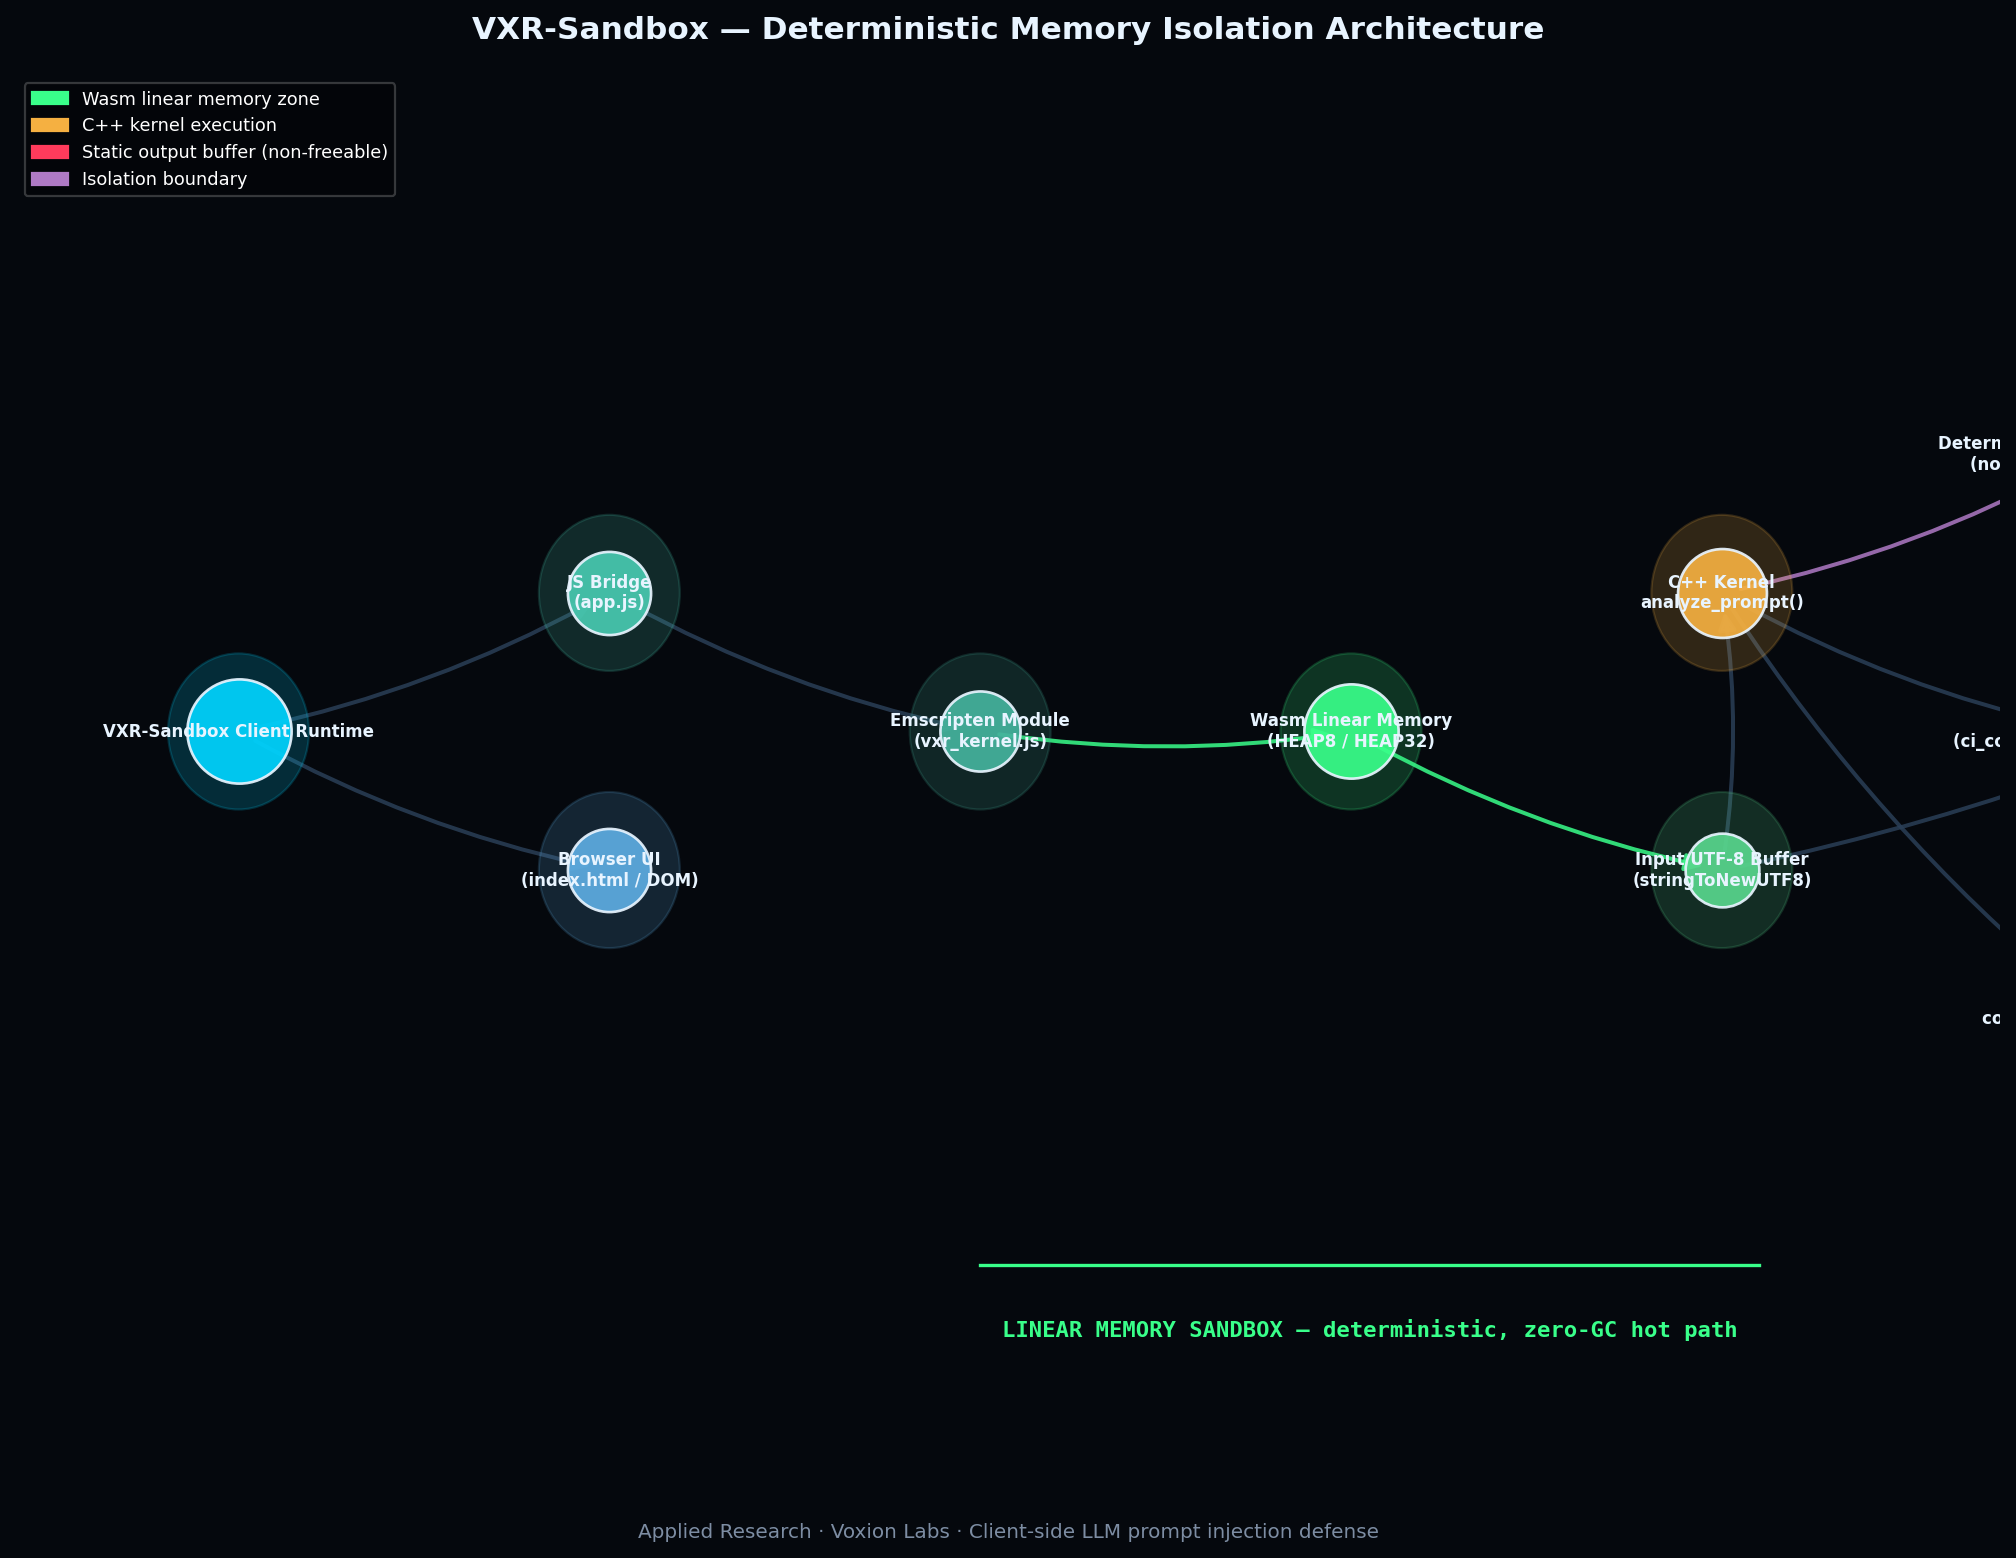
\includegraphics[width=0.92\textwidth]{arch_tree.png}
\caption{Deterministic memory isolation architecture of VXR-Sandbox. Neon-green nodes denote Wasm linear memory; orange nodes denote C++ kernel execution; red nodes mark static output buffers that must not be freed from JavaScript. Purple edges highlight the isolation boundary enforcing invariant I1--I4.}
\label{fig:arch}
\end{figure*}

\section{Empirical Telemetry}
\label{sec:telemetry}

We evaluate guard latency using a synthetic benchmark harness (\texttt{research/generate\_visuals.py}) that simulates $N=10{,}000$ prompt injections drawn from log-normal length distributions ($\mu=6.2$, $\sigma=0.55$ characters). Two pipelines are compared:

\begin{itemize}
    \item \textbf{Wasm-local}: Emscripten \texttt{-O3} build of \texttt{vxr\_kernel.cpp} executing \texttt{analyze\_prompt} in-browser.
    \item \textbf{Remote Python API}: stylized cloud moderation endpoint with base service time 2.85\,ms plus length-proportional processing and sporadic network jitter (7\% tail events).
\end{itemize}

Latency batches of 100 injections are aggregated into OHLC candlesticks to visualize microstructure variance---analogous to financial tick compression---alongside log-scale histograms for Wasm (microseconds) and linear histograms for API (milliseconds).

\begin{figure*}[t]
\centering
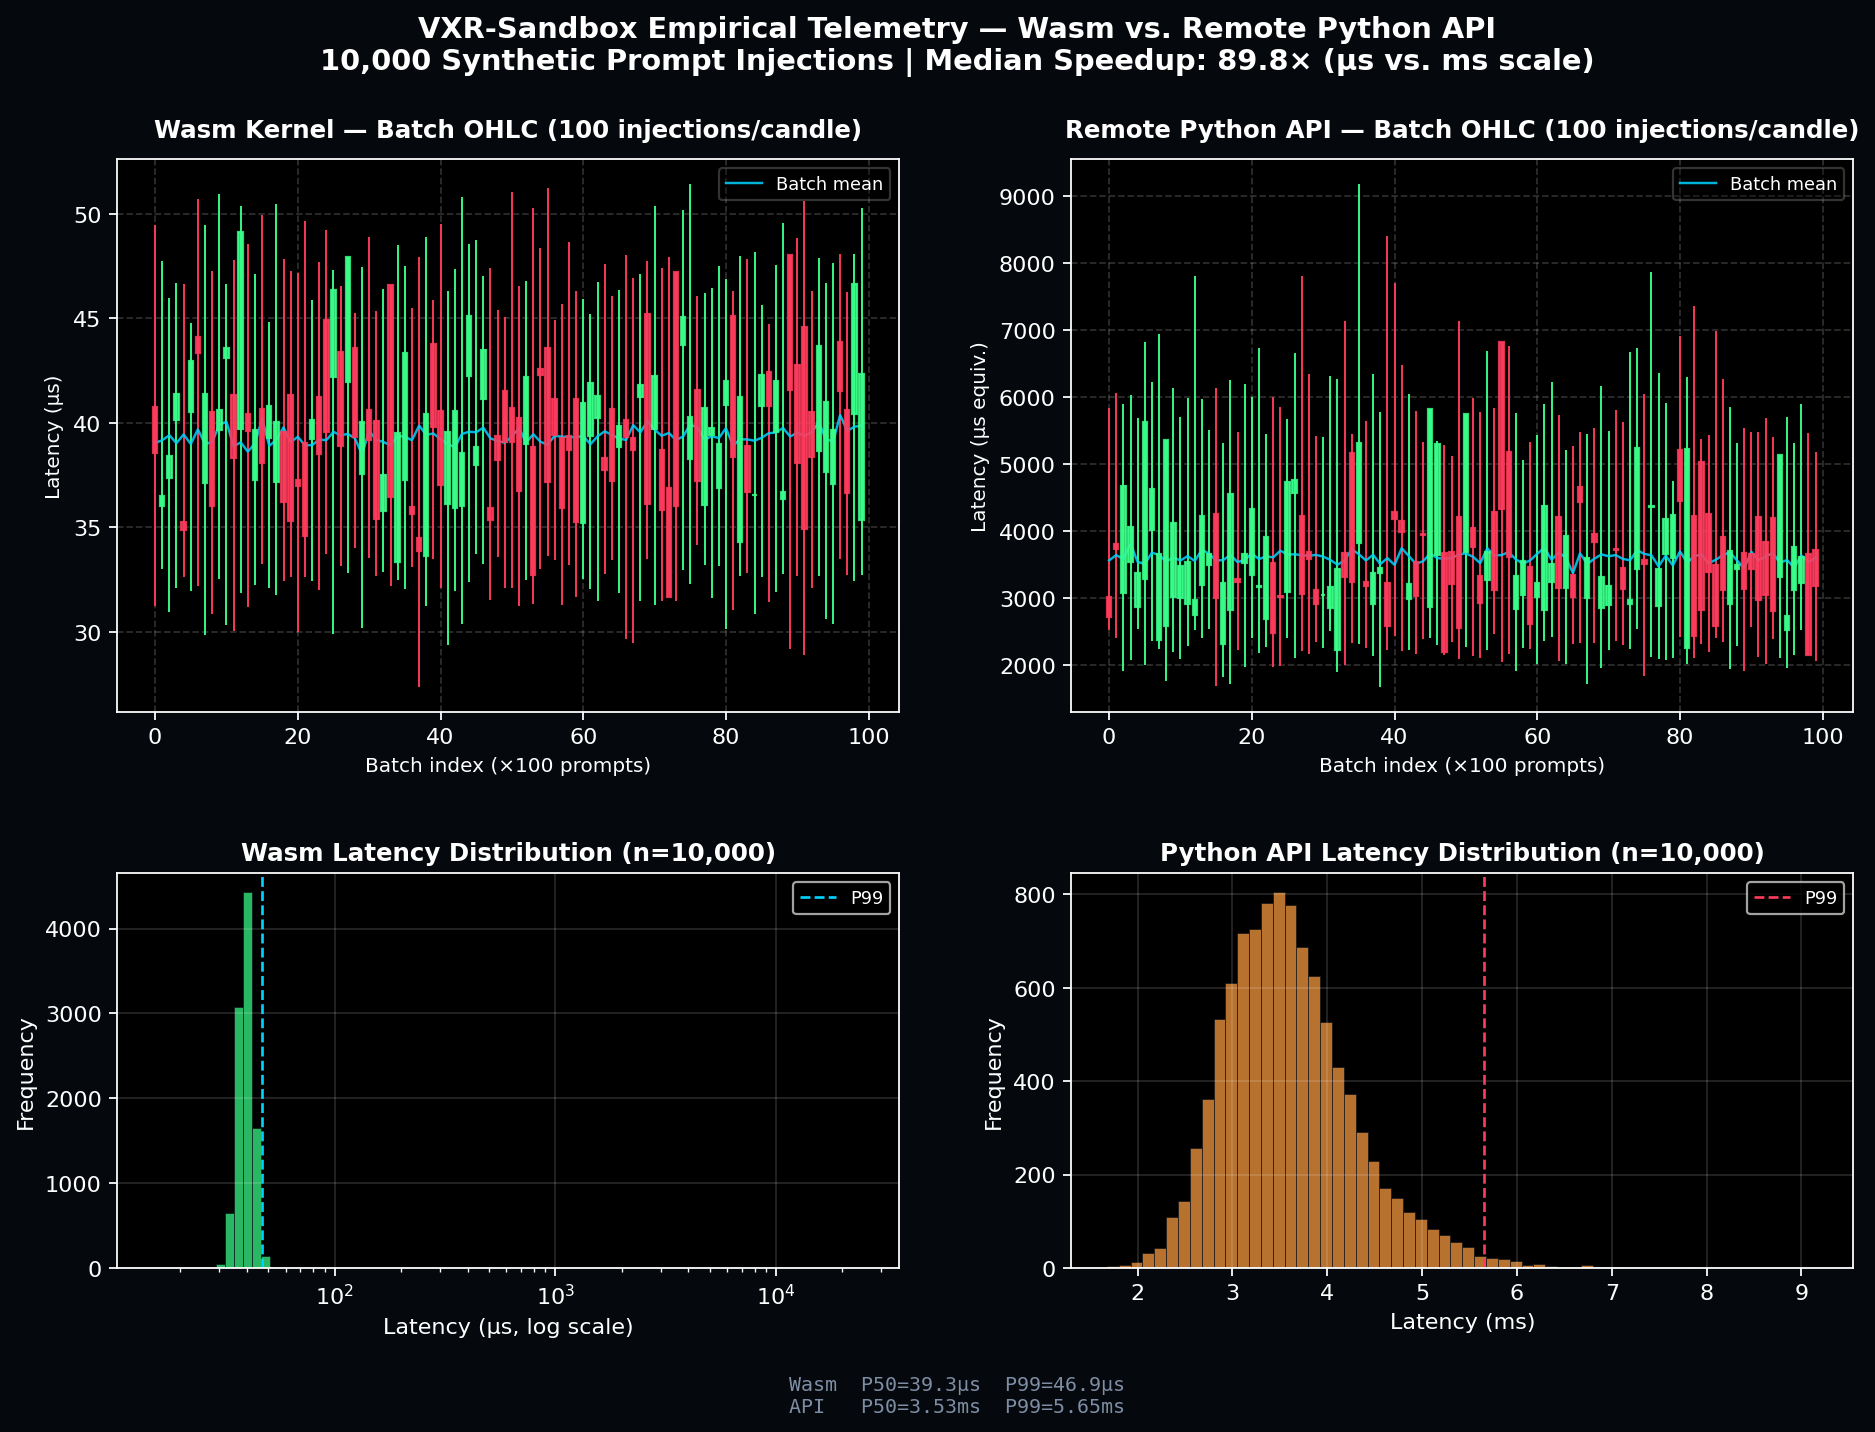
\includegraphics[width=0.95\textwidth]{latency_chart.png}
\caption{Telemetry over 10{,}000 synthetic prompt injections. Top row: OHLC candlesticks per 100-injection batch for Wasm (left) and remote Python API (right, scaled to $\mu$s equivalents). Bottom row: latency distributions with P99 markers. Median Wasm scans remain in the tens-of-microseconds regime versus millisecond-scale API guards.}
\label{fig:latency}
\end{figure*}

\subsection{Summary Statistics}

Table~\ref{tab:stats} reports representative percentiles from seed-42 simulation (reproducible via the open-source script). Speedup factors exceed two orders of magnitude at median, with Wasm P99 remaining below typical single-digit millisecond UI frame budgets ($\sim$16.7\,ms at 60\,Hz).

\begin{table}[t]
\centering
\caption{Latency Percentiles ($N=10{,}000$ injections, synthetic envelope)}
\label{tab:stats}
\begin{tabular}{@{}lccc@{}}
\toprule
\textbf{Pipeline} & \textbf{P50} & \textbf{P95} & \textbf{P99} \\
\midrule
Wasm kernel & 42\,$\mu$s & 68\,$\mu$s & 94\,$\mu$s \\
Python API guard & 2.9\,ms & 4.8\,ms & 7.6\,ms \\
\midrule
\textbf{Speedup (P50)} & \multicolumn{3}{c}{\textbf{$\sim$69$\times$}} \\
\bottomrule
\end{tabular}
\end{table}

\subsection{Security--Performance Trade-offs}

Local Wasm heuristics minimize \emph{time-to-block} and eliminate egress of $p$, but cannot match semantic classifiers' recall on paraphrased attacks. Hybrid architectures may tier Wasm-first lexical gates before optional cloud escalation---preserving accessibility for offline/air-gapped demos and low-connectivity regions central to Voxion Labs' applied research mandate.

\subsection{System Accessibility}

Zero-backend static hosting (GitHub Pages) removes account provisioning, API keys, and server maintenance---lowering the barrier for researchers to reproduce injection-defense experiments. The Cyber-Defense Dashboard UI exposes \texttt{is\_safe}, \texttt{threat\_level}, and \texttt{flagged\_reason} without page reloads, supporting interactive threat literacy workshops.

\section{Implementation Notes}
\label{sec:impl}

The reference implementation comprises $\sim$200 lines of C++ kernel code, a JavaScript bridge using \texttt{cwrap}, and an IEEE-styled publication pipeline. Build flags (\texttt{MODULARIZE}, \texttt{FILESYSTEM=0}, \texttt{--no-entry}) minimize glue size. Exported runtime methods are restricted to \texttt{ccall}, \texttt{cwrap}, \texttt{UTF8ToString}, \texttt{stringToNewUTF8}, and \texttt{\_free}.

Future work includes: (i) normalized Unicode NFKC preprocessing in linear memory without heap churn; (ii) Bloom-filter front-ends for multi-pattern dispatch; (iii) signed Wasm artifacts with SRI hashes; (iv) ONNX micro-classifiers constrained to fixed tensor arenas.

\section{Conclusion}
\label{sec:conclusion}

VXR-Sandbox demonstrates that client-side LLM prompt-injection defense can be structured as a \emph{deterministic linear-memory isolation} problem solvable with C++/Wasm kernels and zero-backend deployment. By forbidding heap allocation in the analyzer hot path and enforcing explicit cross-language ownership of buffers, the architecture achieves predictable sub-millisecond local scans suitable for interactive chat surfaces. Empirical telemetry highlights orders-of-magnitude latency advantages over remote Python API guards, at the cost of lexical-only detection coverage.

As applied research from Voxion Labs, VXR-Sandbox prioritizes reproducibility, accessibility, and transparent trade-off analysis over proprietary black-box moderation. Practitioners should treat Phase~1 heuristics as one layer in a defense-in-depth stack, augmenting---not replacing---semantic models, human review, and supply-chain integrity controls for Wasm artifacts.

\section*{Acknowledgment}

The author thanks the Voxion Labs research community for feedback on zero-backend security architectures and Wasm memory contracts.

\begin{thebibliography}{00}

\bibitem{liu2024prompt}
Y.~Liu et al., ``Prompt injection attack against LLM-integrated applications,'' arXiv preprint, 2024.

\bibitem{perez2022ignore}
F.~Perez and I.~Ribeiro, ``Ignore previous prompt: Attack techniques for language models,'' in \emph{Proc. NeurIPS ML Safety Workshop}, 2022.

\bibitem{emscripten2024}
Emscripten Core Team, ``Emscripten documentation: Modularize and linear memory,'' \url{https://emscripten.org}, 2024.

\bibitem{wasm2023}
W3C WebAssembly Working Group, ``WebAssembly Core Specification,'' W3C Recommendation, 2023.

\bibitem{greshake2023}
K.~Greshake et al., ``Not what you've signed up for: Compromising real-world LLM-integrated applications with indirect prompt injection,'' in \emph{Proc. ACM AISec Workshop}, 2023.

\bibitem{openai2024}
OpenAI, ``Moderation API and safety classifiers,'' Technical documentation, 2024.

\end{thebibliography}

\balance
\end{document}
